\section{When exact pair hulls do not compose}\label{sec:composition}

A solver that relaxes a quadratic expression term by term or pair by pair
works with the variables and products that occur in the model. Even if
every pair were relaxed exactly, gluing the pair hulls on their shared
variables gives in general a weaker set than the hull of the joint graph,
because finitely many shared moments do not determine the distribution of a
shared variable \citep{Lasserre2006,NieDemmel2009,FantuzziFuentes2025}. In
the MINLP literature, \citet[Example~3.8]{Tawarmalani2010} shows that
separate envelopes are weaker than the simultaneous hull because they may
represent the same point by different convex combinations. This section
quantifies the phenomenon for the smallest quadratic case, a path of three
variables with exact pair hulls, and determines exactly when gluing on
$\kappa$ shared moments yields no positive bound. The results explain when
a merged block is stronger than its pairs, and they delimit that advantage.

\subsection{An example on a path}\label{sec:path-example}

Consider variables $x,y,z\in[0,1]$ that interact along the path
$x$--$y$--$z$. Write $m_u$ for the coordinate that represents $u$, $s_u$
for $u^2$ and $p_{uv}$ for $uv$. The exact pair hulls are
\[
H_{xy}=\conv\{(x,y,x^2,y^2,xy):x,y\in[0,1]\},\qquad
H_{yz}=\conv\{(y,z,y^2,z^2,yz):y,z\in[0,1]\},
\]
each described by its semidefinite and RLT constraints
\citep{AnstreicherBurer2010}. Let $R$ be the set of points
\[
(m_x,m_y,m_z,s_x,s_y,s_z,p_{xy},p_{yz})
\]
whose $(x,y)$ and $(y,z)$ parts lie in $H_{xy}$ and $H_{yz}$; the two parts
share $m_y$ and $s_y$. We call $R$ the \emph{glued pair relaxation}. The
joint hull $H=\conv\{(x,y,z,x^2,y^2,z^2,xy,yz):x,y,z\in[0,1]\}$ is
contained in $R$. For a quadratic $\Phi$ in $(x,y,z)$ without the monomial
$xz$, the \emph{linearization} $\operatorname{lin}\Phi$ is the affine
function of these coordinates obtained by replacing each monomial by its
coordinate. Its minimum over $H$ is $\min_{[0,1]^3}\Phi$, and the
difference between this minimum and the minimum over $R$ is the
\emph{gap} of $R$ in the direction of $\Phi$.

\begin{proposition}[A strict gap]\label{prop:path-gap}
The point
\begin{equation}\label{eq:witness}
\bar v=(m_x,m_y,m_z,s_x,s_y,s_z,p_{xy},p_{yz})
=\bigl(\tfrac12,\tfrac12,\tfrac45,\tfrac12,\tfrac5{16},\tfrac45,\tfrac38,\tfrac12\bigr)
\end{equation}
belongs to $R$ but not to $H$. The quadratic
\begin{equation}\label{eq:Phi-example}
\Phi(x,y,z)=\bigl(y-\tfrac14-\tfrac x2\bigr)^2+\bigl(y-\tfrac{5z}8\bigr)^2+x(1-x)+z(1-z)
\end{equation}
has minimum $1/128$ on $[0,1]^3$, attained only at $(1,\tfrac{11}{16},1)$,
while $\operatorname{lin}\Phi(\bar v)=0$. The support inequality
\begin{equation}\label{eq:path-cut}
2s_y-\tfrac12m_y-p_{xy}-\tfrac54p_{yz}+\tfrac54m_x-\tfrac34s_x+m_z-\tfrac{39}{64}s_z\ \ge\ -\tfrac7{128}
\end{equation}
is valid for $H$ and violated by $1/128$ at $\bar v$.
\end{proposition}

\begin{proof}
The measure with mass $\tfrac12$ on each of $(x,y)=(0,\tfrac14)$ and
$(1,\tfrac34)$, and the measure with mass $\tfrac15$ on $(y,z)=(0,0)$ and
$\tfrac45$ on $(\tfrac58,1)$, have the moments
\[
(m_x,m_y,s_x,s_y,p_{xy})=\bigl(\tfrac12,\tfrac12,\tfrac12,\tfrac5{16},\tfrac38\bigr),\qquad
(m_y,m_z,s_y,s_z,p_{yz})=\bigl(\tfrac12,\tfrac45,\tfrac5{16},\tfrac45,\tfrac12\bigr).
\]
They agree on $(m_y,s_y)$, so $\bar v\in R$. The two pair parts of $\Phi$,
$(y-\tfrac14-\tfrac x2)^2+x(1-x)$ and $(y-\tfrac{5z}8)^2+z(1-z)$, vanish on
the supports of the respective measures, so $\operatorname{lin}\Phi(\bar v)=0$.
The minimum is the case $A=\{\tfrac14,\tfrac34\}$, $C=\{0,\tfrac58\}$ of
Theorem~\ref{thm:interleave} below, with $\delta=\tfrac34-\tfrac58=\tfrac18$.
Expanding $\Phi\ge\tfrac1{128}$ gives~\eqref{eq:path-cut}, since the constant
term of $\Phi$ is $\tfrac1{16}$.
\end{proof}

The inequality~\eqref{eq:path-cut} uses only coordinates that occur in the
model; it needs no product $xz$. It is the support inequality of the
three-variable block in the direction of $\Phi$, and both oracles of
Section~\ref{sec:quadratic} compute it exactly.

\subsection{An exact description for a path family}\label{sec:interleave}

The example belongs to a family whose behavior can be described
completely. Fix an interval $[\ell,u]$ for $y$ and two-point sets
$A=\{a_1,a_2\}$ and $C=\{c_1,c_2\}$ in $[\ell,u]$ with $a_1\ne a_2$ and
$c_1\ne c_2$. For weights $\omega_A\ge(a_2-a_1)^2$ and
$\omega_C\ge(c_2-c_1)^2$ let
\begin{equation}\label{eq:family}
\Phi_A(x,y)=\bigl(y-a_1-(a_2-a_1)x\bigr)^2+\omega_Ax(1-x),\qquad
\Phi_C(y,z)=\bigl(y-c_1-(c_2-c_1)z\bigr)^2+\omega_Cz(1-z),
\end{equation}
with $x,z\in[0,1]$, and $\Phi=\Phi_A+\Phi_C$. Define $R$ as above, on the
box $[0,1]\times[\ell,u]\times[0,1]$, and let
$\delta=\min\{\abs{s-t}:s\in A,\ t\in C\}$. The sets $A$ and $C$
\emph{interleave} if they are disjoint and their elements alternate in
sorted order.

\begin{theorem}[Interleaving]\label{thm:interleave}
\begin{enumerate}[label=(\roman*)]
\item The minimum of $\Phi$ over the box is $\delta^2/2$.
\item The minimum of $\operatorname{lin}\Phi$ over $R$ is $0$ if
$A\cap C\ne\emptyset$ or $A$ and $C$ interleave, and $\delta^2/2$ otherwise.
\end{enumerate}
Hence the gap of $R$ in the direction of $\Phi$ is either $0$ or
$\delta^2/2$; it is positive exactly when $A$ and $C$ interleave, and it
then equals $\delta^2/2$.
\end{theorem}

\begin{proof}
Since $\omega_A\ge(a_2-a_1)^2$, the function $\Phi_A(\cdot,y)$ is concave or
affine, so its minimum over $[0,1]$ is attained at $x\in\{0,1\}$, where it
equals $(y-a_1)^2$ or $(y-a_2)^2$. Hence
$\min_{x\in[0,1]}\Phi_A(x,y)=\dist(y,A)^2$, and similarly for $\Phi_C$.

(i) For fixed $y$ the minimum over $x$ and $z$ is
$\min_{s\in A,t\in C}\{(y-s)^2+(y-t)^2\}$, and
$(y-s)^2+(y-t)^2=2(y-\tfrac{s+t}2)^2+\tfrac12(s-t)^2$ with
$\tfrac{s+t}2\in[\ell,u]$.

(ii) A point of $H_{xy}$ is the moment vector of a finitely supported
probability measure $\pi$ on $[0,1]\times[\ell,u]$, and the linearization of
$\Phi_A$ at that point is $\int\Phi_A\,d\pi\ge\int\dist(y,A)^2\,d\nu$, where
$\nu$ is the $y$-marginal of $\pi$; equality holds when $\pi$ puts its mass
at a minimizing $x\in\{0,1\}$ for each $y$. Hence the minimum over $R$ is
the minimum of $\int\dist(y,A)^2\,d\nu_A+\int\dist(y,C)^2\,d\nu_C$ over
probability measures $\nu_A,\nu_C$ on $[\ell,u]$ with equal first and second
moments. It is zero if and only if some measure on $A$ and some measure on
$C$ have equal first two moments, that is, if the chords of the parabola
$\{(t,t^2)\}$ spanned by $A$ and by $C$ meet. Two such chords meet if they
share an endpoint; otherwise, since no three points of a parabola are
collinear and $(t,t^2)$ lies below the chord spanned by $A$ exactly when $t$
lies between $a_1$ and $a_2$, they meet if and only if $A$ and $C$
interleave. When the chords do not meet, $A$ and $C$ are either separated
(one lies below the other) or nested (one lies between the two points of the
other). In both cases Appendix~\ref{app:interleave} gives a polynomial $p$
of degree at most two such that $\dist(y,A)^2-p(y)\ge\eta_A$ and
$\dist(y,C)^2+p(y)\ge\eta_C$ for all $y$, with $\eta_A+\eta_C=\delta^2/2$.
Integrating against $\nu_A$ and $\nu_C$, whose moments of order at most two
agree, shows that the minimum over $R$ is at least $\delta^2/2$, and graph
points show that it is at most $\delta^2/2$.
\end{proof}

\begin{figure}[t]
\centering
\begin{tikzpicture}[scale=4.2]
\begin{scope}
\draw[->] (-0.05,0) -- (0.9,0) node[right] {$t$};
\draw[->] (0,-0.03) -- (0,0.78) node[above] {$t^2$};
\draw[thick,gray,domain=-0.02:0.86,smooth,variable=\t] plot ({\t},{\t*\t});
\coordinate (a1) at (0.25,0.0625); \coordinate (a2) at (0.75,0.5625);
\coordinate (c1) at (0,0); \coordinate (c2) at (0.625,0.390625);
\draw[very thick,blue] (a1) -- (a2);
\draw[very thick,red,dashed] (c1) -- (c2);
\fill[blue] (a1) circle (0.012) node[below right] {$\tfrac14$};
\fill[blue] (a2) circle (0.012) node[right] {$\tfrac34$};
\fill[red] (c1) circle (0.012) node[below left] {$0$};
\fill[red] (c2) circle (0.012) node[above left] {$\tfrac58$};
\fill (0.5,0.3125) circle (0.014);
\node[anchor=north west] at (0.52,0.30) {\small $(\tfrac12,\tfrac5{16})$};
\node at (0.42,0.72) {\small (a) interleaving};
\end{scope}
\begin{scope}[xshift=1.15cm]
\draw[->] (-0.05,0) -- (0.9,0) node[right] {$t$};
\draw[->] (0,-0.03) -- (0,0.78) node[above] {$t^2$};
\draw[thick,gray,domain=-0.02:0.86,smooth,variable=\t] plot ({\t},{\t*\t});
\coordinate (a1) at (0,0); \coordinate (a2) at (0.75,0.5625);
\coordinate (c1) at (0.25,0.0625); \coordinate (c2) at (0.5,0.25);
\draw[very thick,blue] (a1) -- (a2);
\draw[very thick,red,dashed] (c1) -- (c2);
\fill[blue] (a1) circle (0.012) node[below left] {$0$};
\fill[blue] (a2) circle (0.012) node[right] {$\tfrac34$};
\fill[red] (c1) circle (0.012) node[below right] {$\tfrac14$};
\fill[red] (c2) circle (0.012) node[below right] {$\tfrac12$};
\node at (0.42,0.72) {\small (b) nested};
\end{scope}
\end{tikzpicture}
\caption{Moment pairs $(\E y,\E y^2)$ of distributions on a two-point set
form the chord of the parabola between the two points. Solid: $A$;
dashed: $C$. (a) The sets $A=\{\tfrac14,\tfrac34\}$ and $C=\{0,\tfrac58\}$ of
Proposition~\ref{prop:path-gap} interleave,
the chords cross at $(\tfrac12,\tfrac5{16})$, and the glued pair relaxation
has value $0$. (b) Nested sets $A=\{0,\tfrac34\}$ and $C=\{\tfrac14,\tfrac12\}$:
the chords do not meet, and by
Theorem~\ref{thm:interleave} the glued relaxation attains the true minimum
$\delta^2/2$ in the direction of $\Phi$.}
\label{fig:chords}
\end{figure}


Proposition~\ref{prop:path-gap} is the case $[\ell,u]=[0,1]$,
$A=\{\tfrac14,\tfrac34\}$, $C=\{0,\tfrac58\}$ and $\omega_A=\omega_C=1$, with
sorted order $0,\tfrac14,\tfrac58,\tfrac34$. Figure~\ref{fig:chords} shows
what goes wrong. In $R$ the two pairs may represent $y$ by different
distributions that agree only in their first two moments. Each pair places
$y$ on its own preferred two-point set, and whenever the chords cross, the
two distributions have the same mean and second moment. The theorem
concerns the directions $\Phi$ of the family~\eqref{eq:family}; in other
directions on the path the gap can take other values, and
Proposition~\ref{prop:gain}(ii) expresses it for every direction.

\subsection{Matching more moments}\label{sec:k-moments}

The same mechanism defeats any interface that identifies a fixed finite
number of moments of the shared variable. Let $X_L$ and $X_R$ be compact
sets of points $(x,y)$ and $(y,z)$, with $y$ scalar, and let $H_L$ and $H_R$
be the convex hulls of continuous feature maps on them whose first $\kappa$
coordinates are $y,y^2,\dots,y^\kappa$; the other local features are
arbitrary. Let $R_\kappa$ be the set of pairs of points of $H_L$ and $H_R$
that agree in these $\kappa$ coordinates. Let $\Phi_L\ge0$ on $X_L$ and
$\Phi_R\ge0$ on $X_R$ be affine functions of the local features, with zero
sets $Z_L$ and $Z_R$, and let $A$ and $C$ be the projections of $Z_L$ and
$Z_R$ onto $y$. For disjoint compact $A,C\subset\R$, the \emph{alternation
number} $\operatorname{alt}(A,C)$ is the largest $r$ for which there are
points $t_0<\dots<t_r$ of $A\cup C$ with consecutive points in different
sets, and $\operatorname{alt}(A,C)=0$ if $A\cup C$ has at most one point.

\begin{theorem}[Alternation]\label{thm:alternation}
Suppose $A$ and $C$ are disjoint, so that $\Phi_L+\Phi_R>0$ at every point
$(x,y,z)$ with $(x,y)\in X_L$ and $(y,z)\in X_R$. The linearization of
$\Phi_L+\Phi_R$ vanishes at some point of $R_\kappa$ if and only if
$\operatorname{alt}(A,C)\ge\kappa+1$. In particular, gluing on $\kappa$
moments always gives a positive bound when $\abs A+\abs C\le\kappa+1$, and,
for finite sets with $\abs A+\abs C=\kappa+2$, gives the bound zero exactly
when $A$ and $C$ alternate.
\end{theorem}

\begin{proof}
As in the proof of Theorem~\ref{thm:interleave}, the linearization vanishes
at a point of $R_\kappa$ if and only if there are probability measures on
$A$ and on $C$ with equal moments of orders $1,\dots,\kappa$; these measures
lift to $Z_L$ and $Z_R$ atom by atom. If $\operatorname{alt}(A,C)=r\le\kappa$,
there is a polynomial of degree $r$ that is positive on $A$ and negative on
$C$ (Appendix~\ref{app:alternation}), and its integrals against two such
measures would have to be equal, a contradiction. If
$\operatorname{alt}(A,C)\ge\kappa+1$, take an alternating chain
$t_0<\dots<t_{\kappa+1}$ and the weights $w_i=\prod_{j\ne i}(t_i-t_j)^{-1}$
of the divided difference of order $\kappa+1$. They annihilate all
polynomials of degree at most $\kappa$, and their signs alternate, so their
positive and negative parts, normalized, are probability measures on the
$A$-points and on the $C$-points with equal moments of orders
$0,\dots,\kappa$.
\end{proof}

For finite $A$ and $C$ the criterion is the classical description of Radon
partitions of points on the moment curve: the convex hulls of
$\{(t,\dots,t^\kappa):t\in A\}$ and $\{(t,\dots,t^\kappa):t\in C\}$ meet
exactly when $A$ and $C$ alternate at least $\kappa+1$ times
\citep{Breen1973}. By Gordan's alternative it is equivalent to the fact that
the least degree of a polynomial that is positive on $A$ and negative on $C$
is $\operatorname{alt}(A,C)$, which rests on the sign-change properties of
Chebyshev systems \citep{KarlinStudden1966}. Theorem~\ref{thm:interleave}(ii)
is the case $\kappa=2$. What the theorem adds is its reading as a criterion
for gluing interfaces.

Theorem~\ref{thm:alternation} characterizes when the glued bound is zero,
not when it is exact. For $\kappa\ge3$ the glued bound can lie strictly
between $0$ and the minimum. For $\Phi_L=(y-2x)^2+4x(1-x)$ and
$\Phi_R=(y-1-2z)^2+4z(1-z)$ with $x,z\in[0,1]$ and $y\in[0,3]$ we have
$A=\{0,2\}$, $C=\{1,3\}$ and $\operatorname{alt}(A,C)=3$, so gluing on
$\kappa=3$ moments gives a positive bound. The probability measure $\nu_A$
with masses $\tfrac{57}{112}$ and $\tfrac{55}{112}$ at $\tfrac{15}{32}$ and
$\tfrac{57}{32}$, and the probability measure $\nu_C$ with masses
$\tfrac{22}{117}$, $\tfrac{1045}{1456}$ and $\tfrac{95}{1008}$ at $0$,
$\tfrac{39}{32}$ and $\tfrac{81}{32}$, have equal moments of orders up to
three, and
$\int\dist(y,A)^2d\nu_A+\int\dist(y,C)^2d\nu_C=6103/16128\approx0.378$,
whereas $\min(\Phi_L+\Phi_R)=1/2$. The dichotomy of
Theorem~\ref{thm:interleave} is therefore specific to two shared moments and
two-point sets. For every $\kappa$, however, some quadratic configuration has
a full gap.

\begin{proposition}[A full gap for every $\kappa$]\label{prop:full-gap}
Let $\kappa\ge1$ and choose $r\ge1$ with $\kappa\le2^{r+1}-2$. On
$x,z\in[0,1]^r$ and $y\in[0,2^{r+1}-1]$ let
\[
\Phi_L=\Bigl(y-\sum_{j=1}^r2^jx_j\Bigr)^2+\sum_{j=1}^r4^jx_j(1-x_j),\qquad
\Phi_R=\Bigl(y-1-\sum_{j=1}^r2^jz_j\Bigr)^2+\sum_{j=1}^r4^jz_j(1-z_j).
\]
Let $H_L$ be the convex hull of the features $y,\dots,y^{\max\{\kappa,2\}}$,
$x_j$, $yx_j$ and $x_ix_j$ $(i<j)$ over $[0,1]^r\times[0,2^{r+1}-1]$, and $H_R$
the analogous hull in $(y,z)$. Then $\min(\Phi_L+\Phi_R)=1/2$, while the
linearization of $\Phi_L+\Phi_R$ vanishes at a point of $R_\kappa$.
\end{proposition}

\begin{proof}
The coefficient of $x_j^2$ in $\Phi_L$ is $4^j-4^j=0$, so $\Phi_L$ is affine
in the features and multilinear in $x$. Its minimum over $x$ is therefore
attained at a vertex, where it equals $(y-\sum_{j\in J}2^j)^2$ for a subset
$J$; hence $\min_x\Phi_L=\dist(y,A)^2$ with $A=\{0,2,\dots,2^{r+1}-2\}$, and
similarly $\min_z\Phi_R=\dist(y,C)^2$ with $C=\{1,3,\dots,2^{r+1}-1\}$. By the
argument of Theorem~\ref{thm:interleave}(i), with $\delta=1$, the minimum is
$1/2$. The points $0,1,\dots,\kappa+1$ alternate between $A$ and $C$, so
Theorem~\ref{thm:alternation} applies; explicitly, the binomial weights
$\binom{\kappa+1}i2^{-\kappa}$ on the even and on the odd integers
$i\le\kappa+1$ have equal moments of orders up to $\kappa$.
\end{proof}

Thus no fixed number of shared moments makes the gluing exact, even for
quadratic blocks, and the relative gap can be $100\%$. As $\kappa\to\infty$
the glued bounds do converge to the true minimum, because measures on a
compact interval are determined by their moments and measures with equal
marginals glue \citep[Lemma~6.3]{Lasserre2006}; the convergence is not
uniform over instances.

\subsection{Relation to known results}\label{sec:composition-literature}

Several earlier examples show that sparse relaxations on a path can be
strictly weaker than dense ones. \citet[Example~3.5]{NieDemmel2009} give a
numerical quartic example, and \citet[Example~6.7]{NieQuTangZhang2026} a
box-constrained quartic for which the sparse moment hierarchy is never
tight. Finite gluing results require rank or flatness conditions on the
overlaps \citep[Theorem~3.7]{Lasserre2006}, \citep{FantuzziFuentes2025}. For
sparse quadratically constrained problems, \citet{KojimaKimArima2026} assemble
exactness of the semidefinite relaxation from exact clique-wise subproblems;
they assume that maximal cliques meet in at most one node, because shared
off-diagonal entries impose product conditions that local exactness cannot
control \citep[Section~3.3]{KojimaKimArima2026}, and the same block-clique
structure makes doubly nonnegative relaxations exact
\citep{KimKojimaToh2020}. In our path, the homogenized cliques $\{1,x,y\}$ and
$\{1,y,z\}$ share the off-diagonal entry $m_y$ as well as $s_y$, and
Proposition~\ref{prop:path-gap} shows that this obstruction occurs even when
the local relaxations are exact hulls.
For quadratic problems with sign-oriented squares,
\citet[Corollary~1]{DeyKhajavirad2025} decompose the convex hull across a
complete separator that carries no positive square term (no ``plus loop''),
and \citet{Khajavirad2026} builds on this decomposition.
Proposition~\ref{prop:path-gap} shows that the hypothesis cannot be dropped
even for a path of three variables with a single plus loop at the center:
the reduced objective
$2y^2-\tfrac12y-xy-\tfrac54yz+\tfrac1{16}+\tfrac12x+\tfrac{25}{64}z$, which
equals $\Phi$ at binary leaves, has the same witness and the same gap $1/128$.
Their stable-set theorem \citep[Theorem~2 and Corollary~4]{DeyKhajavirad2025} still gives an
exact extended formulation for this sign pattern, because the plus-loop node
$y$ is a stable set, but it adds the products among the neighbors of $y$,
here the nonedge product $xz$; this matches the next paragraph. To our
knowledge, a degree-two example with exact pair hulls, an exact rational gap
and a separating cut in the existing coordinates, the value $\delta^2/2$ of
the gap in Theorem~\ref{thm:interleave}, and the use of the alternation
criterion to decide when a $\kappa$-moment interface gives no positive bound
have not been given before.

On a three-variable path, the advantage of the joint block over its pairs
does not extend to dense relaxations. Sparse and dense Shor relaxations \citep{Shor1987} coincide
for chordal sparsity patterns, because a partial positive semidefinite
matrix with a chordal pattern has a positive semidefinite completion
\citep{GroneEtAl1984,WakiEtAl2006,Laurent2009}. Hence $R$ is the projection of
the dense moment relaxation of $(1,x,y,z)$ with the RLT inequalities
\citep{SheraliAdams1990,SheraliTuncbilek1992} of the edges and squares, and
what closes the gap must constrain the nonedge product $p_{xz}$, for example
through its McCormick inequalities. On the whole family~\eqref{eq:family}, with
$\xi_A=y-a_1-(a_2-a_1)x$ and $\xi_C=y-c_1-(c_2-c_1)z$,
\begin{equation}\label{eq:sdp-identity}
\Phi-\frac{\delta^2}2=\frac{(\xi_A+\xi_C)^2}2+\sum_{i,j\in\{0,1\}}F_{ij}\,\ell_{ij}(x,z)
+\Bigl(\omega_A-\frac{(a_2-a_1)^2}2\Bigr)x(1-x)+\Bigl(\omega_C-\frac{(c_2-c_1)^2}2\Bigr)z(1-z),
\end{equation}
where $\ell_{00}=(1-x)(1-z)$, $\ell_{10}=x(1-z)$, $\ell_{01}=(1-x)z$,
$\ell_{11}=xz$, and $F_{ij}=\tfrac12\bigl((c_{j+1}-a_{i+1})^2-\delta^2\bigr)\ge0$.
The linearized $\ell_{ij}$ are the McCormick expressions of the product $xz$,
the linearized $(\xi_A+\xi_C)^2$ is a quadratic form in the dense moment matrix
of $(1,x,y,z)$, and the last two terms are nonnegative on the pair hulls.
Hence the dense moment matrix together with the McCormick inequalities of
the nonedge product $xz$ proves $\Phi\ge\delta^2/2$ for every member of the
family, and neither ingredient alone suffices (Appendix~\ref{app:sdp}). This
is a special case of a theorem of \citet[Theorem~1]{BurerNatarajanWillemsen2025}:
for box-constrained quadratic programs in at most three variables whose
off-diagonal coefficients are nonpositive, the Shor relaxation with the RLT
upper bounds is exact. On a path $x$--$y$--$z$ over a box, replacing $x$ by
its complement or $z$ by its complement where necessary makes the
coefficients of $xy$ and $yz$ nonpositive, the coefficient of $xz$ stays zero,
and complementation maps McCormick inequalities to McCormick inequalities.
The dense moment relaxation with the McCormick inequalities of all products,
including $xz$, is therefore exact for every quadratic objective on a
three-variable path over a box, and~\eqref{eq:sdp-identity} is an explicit
certificate for the family. The support inequality~\eqref{eq:path-cut}
attains the same bound without the coordinate $p_{xz}$ and without a
semidefinite constraint. That matters in practice, because solvers relax the
products present in the model and rarely add new ones; but on three variables
the advantage is one of representation, not of strength over such
relaxations.

The restriction to three variables matters. From four variables on, the dense
relaxation with the McCormick inequalities of all products is no longer exact
for every objective, and joint blocks can be strictly stronger. The objective of
\citet[Example~4]{BurerNatarajanWillemsen2025} is $x\T Qx+c\T x$ with the
tridiagonal matrix $Q$ that has diagonal $(8,25,25,8)$ and off-diagonal
entries $-14,-25,-14$, and with $c=(12,29,0,0)$; its interaction graph is the
path $x_1$--$x_2$--$x_3$--$x_4$. Its minimum over $[0,1]^4$ is $0$
(Theorem~\ref{thm:polytope}), whereas the dense relaxation contains a rational
point with objective value $-109/1024$ \citep[Section~6.4]{BurerNatarajanWillemsen2025};
numerically its value is about $-0.122$, and that of the glued pair hulls of
the three edges about $-1.454$. The instances of Proposition~\ref{prop:full-gap}
behave even worse: for $r=2$ and $r=3$ (five and seven variables) the dense
relaxation contains rational points with objective values below $10^{-6}$,
which we verified exactly, whereas the minimum is $1/2$; for $r=1$ (three
variables) it attains $1/2$, as the theorem above predicts. In both cases the
support inequality of the joint block in the direction of the objective uses
only the coordinates of the model and attains the minimum. For blocks of four
or more variables, joint support cuts can therefore be much stronger than dense
first-level relaxations, not only more economical.

\subsection{When gluing is exact, and the gain from merging}\label{sec:gluing}

Gluing is exact when the shared coordinates determine the shared
distribution. Under a running-intersection decomposition, local measures
with equal full marginals on the separators glue to a global measure
\citep{Vorobev1962,Lasserre2006}, and \citet[Corollary~3.10]{Tawarmalani2010}
glues two functions that share a variable when their inclusion certificates
have equal marginals of that variable. If the separator takes finitely many
known values $t_1,\dots,t_N$, its moments of orders $0,\dots,N-1$ determine
its distribution through a Vandermonde system; for a binary separator the
mean suffices. This is why the McCormick inequalities describe the convex
hull of a pure bilinear function on a forest over the unit box
\citep[Proposition~8]{Padberg1989}: the extreme points are binary, the
McCormick inequalities of an edge are the nonnegativity of the four joint
probabilities of its endpoints, and adjacent edges share a binary variable
whose distribution is fixed by its mean. Square terms break this argument,
because they let a fractional mean be realized by continuous distributions,
as in~\eqref{eq:witness}.

The gain from merging pair directions into one star direction can be
computed exactly, and it is related to the glued relaxation by a
re-splitting of the center terms. Part~(ii) of the next proposition is the
Lagrangian-decomposition duality \citep{Geoffrion1974,GuignardKim1987} applied
to the pair hulls, with the shared moments $(m_y,s_y)$ as copied variables; in the
language of sparse moment relaxations, it says that the glued bound is the best
split of the objective with an interface polynomial of degree two in $y$
\citep{GrimmNetzerSchweighofer2007}, \citep[Theorem~3.1]{NieQuTangZhang2026}.
What we add is that exact pair and star minima evaluate both sides.

\begin{proposition}[Gain from merging]\label{prop:gain}
Let $P_i\subset\R^2$ be rational polytopes in the variables $(y,x_i)$,
$i=1,\dots,k$, whose star domain $\Omega=\{(y,x):(y,x_i)\in P_i\text{ for all }i\}$
is nonempty, and let $q_i(y,x_i)$ be rational quadratics. Put
$\beta_i=\min_{P_i}q_i$, $\beta^\ast=\min_\Omega\sum_iq_i$ and
$\Delta=\beta^\ast-\sum_i\beta_i$.
\begin{enumerate}[label=(\roman*)]
\item $\Delta\ge0$ is the largest constant $c$ such that
$\sum_iq_i\ge\sum_i\beta_i+c$ on $\Omega$, and $\Delta>0$ if and only if the
projections onto $y$ of the sets $\argmin_{P_i}q_i$ have empty common
intersection.
\item Let $R_\Omega$ be the set of $k$-tuples of points of the pair hulls
$\conv\{(y,x_i,y^2,yx_i,x_i^2):(y,x_i)\in P_i\}$ that agree in $(m_y,s_y)$.
Then $\beta^\ast-\min_{R_\Omega}\sum_i\operatorname{lin}q_i=\inf\Delta'$, where
the infimum is over all re-splittings $q_i'=q_i+\alpha_iy+\gamma_iy^2$ with
$\sum_i\alpha_i=\sum_i\gamma_i=0$, and $\Delta'$ is computed as $\Delta$ for
the $q_i'$.
\end{enumerate}
\end{proposition}

\begin{proof}
(i) Clearly $\sum_iq_i\ge\sum_i\beta_i$ on $\Omega$, and $\beta^\ast$ is the
best constant in that direction. If some $\bar y$ lies in every projection,
choose $x_i$ with $(\bar y,x_i)\in\argmin_{P_i}q_i$; the assembled point lies
in $\Omega$ and attains $\sum_i\beta_i$. Conversely, if $\Delta=0$, a minimizer
over $\Omega$ minimizes every $q_i$, so its $y$-coordinate lies in every
projection.

(ii) A re-splitting does not change $\sum_iq_i$, so $\beta^\ast$ is the same for
all of them. The set $R_\Omega$ is the intersection of the compact convex
product of the pair hulls with the linear equations
$m_y^{(i)}=m_y^{(1)}$ and $s_y^{(i)}=s_y^{(1)}$ for $i\ge2$, and it is
nonempty because $\Omega$ is. Attach multipliers to these equations. Their
Lagrangian is bilinear, and by the minimax theorem for a compact convex
set \citep{Sion1958} the minimum of $\sum_i\operatorname{lin}q_i$ over
$R_\Omega$ equals the supremum over the multipliers of the minimum of the
Lagrangian over the product of the pair hulls. A choice of multipliers is
exactly a re-splitting with $\sum_i\alpha_i=\sum_i\gamma_i=0$, and the minimum
of the Lagrangian then separates into $\sum_i\min_{P_i}q_i'=\sum_i\beta_i'$.
Hence $\min_{R_\Omega}\sum_i\operatorname{lin}q_i=\sup\sum_i\beta'_i$, which is
the claim.
\end{proof}

Both $\beta_i$ and $\beta^\ast$ are computed exactly by the algorithms of
Section~\ref{sec:quadratic}; in Proposition~\ref{prop:path-gap} both pair
minima are zero and $\Delta=1/128$. Since each $\beta_i'$ is a minimum of
functions that are affine in $(\alpha_i,\gamma_i)$, part~(ii) turns the gap of
the glued relaxation in any direction into the maximization of a concave
function of $2(k-1)$ parameters whose oracle is the pair minimum. The quantity $\Delta$ compares the merged
cut with separately added pair cuts for one decomposition, and the gap to
the glued relaxation is its infimum over re-splittings;
Appendix~\ref{app:gain-examples} gives two examples, one in which a
re-splitting removes the whole gain and one in which pairwise intersections of
the projections in~(i) do not suffice. The proposition is a diagnostic
for a proposed merge; it does not say which directions to merge or whether
merging pays off in a solver.
